\pagebreak
\section{Introduction}

    \subsection{Overview}
    A flow that is incompressible and irrotational can be modeled by Laplace’s equation for a scalar velocity potential. In two dimensions, an equivalent formulation is obtained using a stream function, $\psi(x, y)$, from which the velocity components are given by

    \begin{equation}
        u = \frac{\partial \psi}{\partial y},\qquad v = -\frac{\partial \psi}{\partial x}
        \label{eqn:velocity}
    \end{equation}\myequations{Stream Function Velocity Components}

    With this definition, continuity is automatically satisfied. Requiring the flow to be irrotational leads to Laplace’s equation for $\psi$,

    \begin{equation}
        \nabla^2\psi = 0
        \label{eqn:laplace_eqn}
    \end{equation}\myequations{Laplace's Equation}

    In this project, I will be solving for two-dimensional potential flow around a square, as illustrated in Figure \ref{fig:solution}.

    \begin{figure}[h]
        \centering
        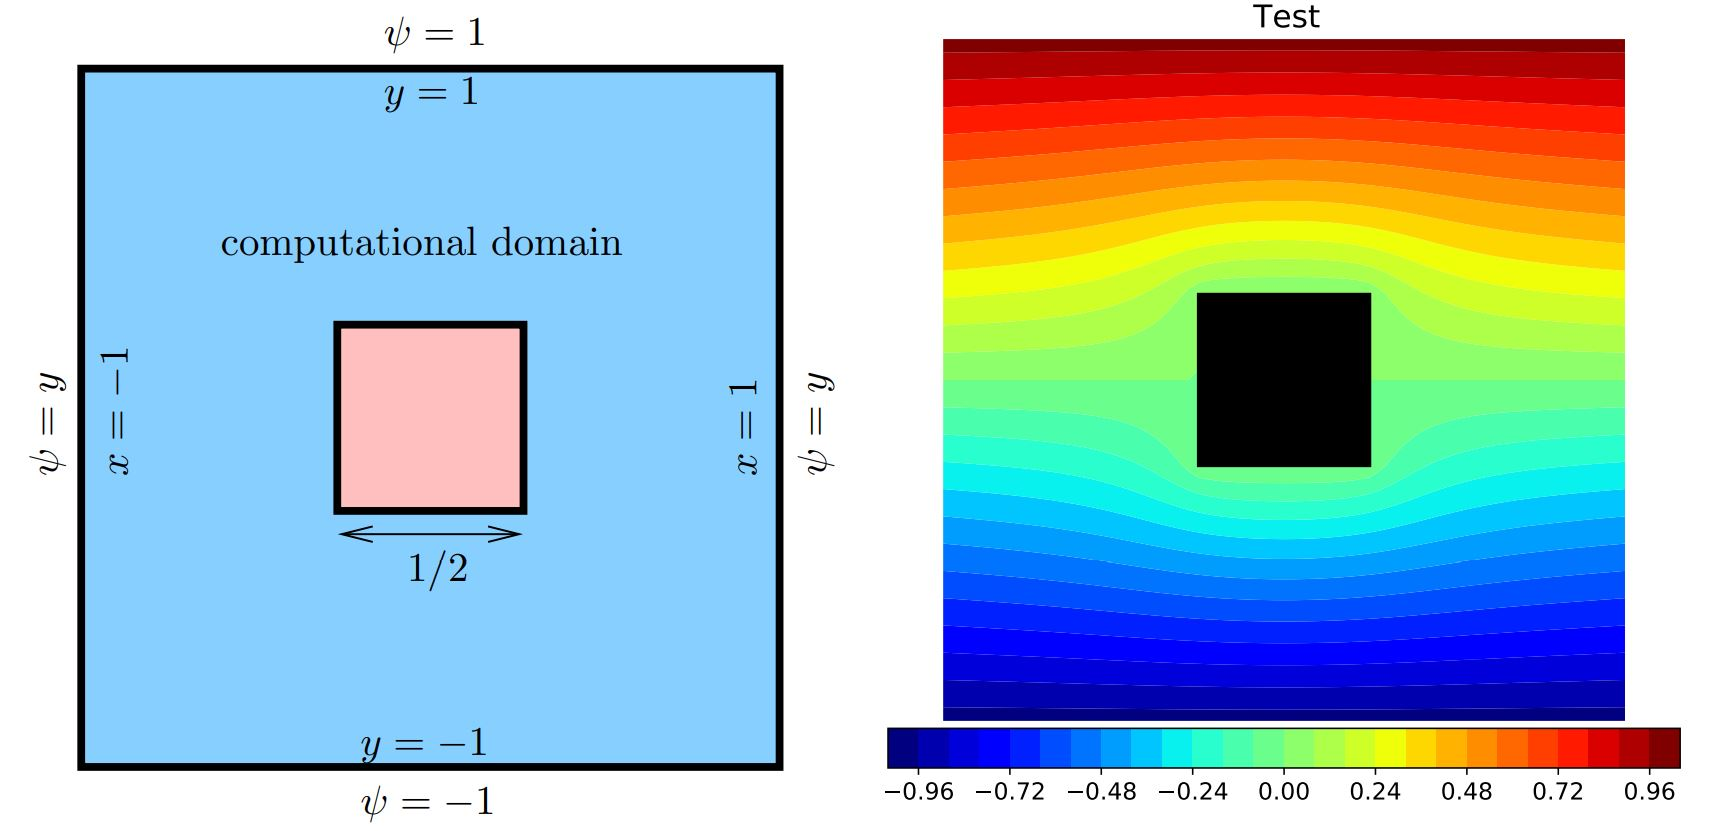
\includegraphics[width = 0.9\linewidth]{rep/solution.JPG}
        \caption[Solution of Potential Flow Around a Square]{Solution of potential flow around a square, using a stream function, $\psi(x, y)$.}
        \label{fig:solution}
    \end{figure}

    The computational domain is a square, $(x, y) \in [-1, 1]^2$ , and the boundary conditions are Dirichlet. On the bottom and top walls, $\psi$ is set to -1 and +1, respectively, and on the sides, $\psi$ is set to $y$. The inner square, of side length $\frac{1}{2}$ and placed in the center of the outer square, presents an obstacle to the flow, and by symmetry it corresponds to a streamline on which $\psi = 0$.


    \pagebreak
    \subsection{Discretization}
    I will use a finite-difference method to solve Equation \ref{eqn:laplace_eqn} on the computational domain. The grid consists of a lattice of $(N + 1)^2$ points, as shown in Figure \ref{fig:fea_grid}. Some of these points are on the boundary, and some are inside the inner square, hence outside the computational domain. It is up to me to decide how best to deal with these points. N is the number of intervals across the entire domain, so that the spacing is $\Delta x = \Delta y = h = 2/N$.

    \begin{figure}[h]
        \centering
        

\tikzset{every picture/.style={line width=0.75pt}} %set default line width to 0.75pt        

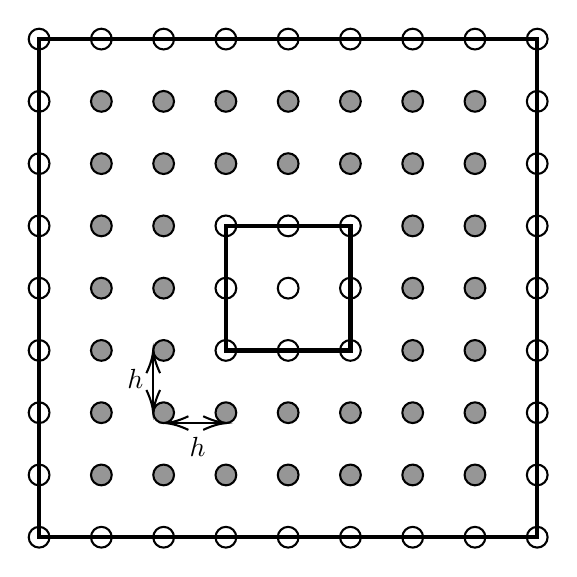
\begin{tikzpicture}[x=0.75pt,y=0.75pt,yscale=-1,xscale=1]
%uncomment if require: \path (0,300); %set diagram left start at 0, and has height of 300

%Shape: Square [id:dp9525805557604268] 
\draw  [line width=1.5]  (295,115) -- (355,115) -- (355,175) -- (295,175) -- cycle ;
%Shape: Circle [id:dp6125642710234998] 
\draw   (290,175) .. controls (290,172.24) and (292.24,170) .. (295,170) .. controls (297.76,170) and (300,172.24) .. (300,175) .. controls (300,177.76) and (297.76,180) .. (295,180) .. controls (292.24,180) and (290,177.76) .. (290,175) -- cycle ;
%Shape: Circle [id:dp6162342043666726] 
\draw   (290,115) .. controls (290,112.24) and (292.24,110) .. (295,110) .. controls (297.76,110) and (300,112.24) .. (300,115) .. controls (300,117.76) and (297.76,120) .. (295,120) .. controls (292.24,120) and (290,117.76) .. (290,115) -- cycle ;
%Shape: Circle [id:dp0847538831868413] 
\draw   (290,145) .. controls (290,142.24) and (292.24,140) .. (295,140) .. controls (297.76,140) and (300,142.24) .. (300,145) .. controls (300,147.76) and (297.76,150) .. (295,150) .. controls (292.24,150) and (290,147.76) .. (290,145) -- cycle ;
%Shape: Circle [id:dp630432347755755] 
\draw   (320,115) .. controls (320,112.24) and (322.24,110) .. (325,110) .. controls (327.76,110) and (330,112.24) .. (330,115) .. controls (330,117.76) and (327.76,120) .. (325,120) .. controls (322.24,120) and (320,117.76) .. (320,115) -- cycle ;
%Shape: Circle [id:dp3960425770816389] 
\draw   (350,145) .. controls (350,142.24) and (352.24,140) .. (355,140) .. controls (357.76,140) and (360,142.24) .. (360,145) .. controls (360,147.76) and (357.76,150) .. (355,150) .. controls (352.24,150) and (350,147.76) .. (350,145) -- cycle ;
%Shape: Circle [id:dp6499473755155605] 
\draw   (320,145) .. controls (320,142.24) and (322.24,140) .. (325,140) .. controls (327.76,140) and (330,142.24) .. (330,145) .. controls (330,147.76) and (327.76,150) .. (325,150) .. controls (322.24,150) and (320,147.76) .. (320,145) -- cycle ;
%Shape: Circle [id:dp1431238040197349] 
\draw   (350,175) .. controls (350,172.24) and (352.24,170) .. (355,170) .. controls (357.76,170) and (360,172.24) .. (360,175) .. controls (360,177.76) and (357.76,180) .. (355,180) .. controls (352.24,180) and (350,177.76) .. (350,175) -- cycle ;
%Shape: Circle [id:dp967579145229569] 
\draw   (320,175) .. controls (320,172.24) and (322.24,170) .. (325,170) .. controls (327.76,170) and (330,172.24) .. (330,175) .. controls (330,177.76) and (327.76,180) .. (325,180) .. controls (322.24,180) and (320,177.76) .. (320,175) -- cycle ;
%Shape: Circle [id:dp5228395860833328] 
\draw   (350,115) .. controls (350,112.24) and (352.24,110) .. (355,110) .. controls (357.76,110) and (360,112.24) .. (360,115) .. controls (360,117.76) and (357.76,120) .. (355,120) .. controls (352.24,120) and (350,117.76) .. (350,115) -- cycle ;
%Shape: Square [id:dp7909173347283065] 
\draw  [line width=1.5]  (205,25) -- (445,25) -- (445,265) -- (205,265) -- cycle ;
%Shape: Circle [id:dp45003349630086165] 
\draw  [fill={rgb, 255:red, 150; green, 150; blue, 150 }  ,fill opacity=1 ] (350,205) .. controls (350,202.24) and (352.24,200) .. (355,200) .. controls (357.76,200) and (360,202.24) .. (360,205) .. controls (360,207.76) and (357.76,210) .. (355,210) .. controls (352.24,210) and (350,207.76) .. (350,205) -- cycle ;
%Shape: Circle [id:dp3012074954118391] 
\draw  [fill={rgb, 255:red, 150; green, 150; blue, 150 }  ,fill opacity=1 ] (320,205) .. controls (320,202.24) and (322.24,200) .. (325,200) .. controls (327.76,200) and (330,202.24) .. (330,205) .. controls (330,207.76) and (327.76,210) .. (325,210) .. controls (322.24,210) and (320,207.76) .. (320,205) -- cycle ;
%Shape: Circle [id:dp5071474511333922] 
\draw  [fill={rgb, 255:red, 150; green, 150; blue, 150 }  ,fill opacity=1 ] (290,205) .. controls (290,202.24) and (292.24,200) .. (295,200) .. controls (297.76,200) and (300,202.24) .. (300,205) .. controls (300,207.76) and (297.76,210) .. (295,210) .. controls (292.24,210) and (290,207.76) .. (290,205) -- cycle ;
%Shape: Circle [id:dp00997904028524843] 
\draw  [fill={rgb, 255:red, 150; green, 150; blue, 150 }  ,fill opacity=1 ] (410,205) .. controls (410,202.24) and (412.24,200) .. (415,200) .. controls (417.76,200) and (420,202.24) .. (420,205) .. controls (420,207.76) and (417.76,210) .. (415,210) .. controls (412.24,210) and (410,207.76) .. (410,205) -- cycle ;
%Shape: Circle [id:dp2857072444657158] 
\draw  [fill={rgb, 255:red, 150; green, 150; blue, 150 }  ,fill opacity=1 ] (380,205) .. controls (380,202.24) and (382.24,200) .. (385,200) .. controls (387.76,200) and (390,202.24) .. (390,205) .. controls (390,207.76) and (387.76,210) .. (385,210) .. controls (382.24,210) and (380,207.76) .. (380,205) -- cycle ;
%Shape: Circle [id:dp44003374769841597] 
\draw   (200,205) .. controls (200,202.24) and (202.24,200) .. (205,200) .. controls (207.76,200) and (210,202.24) .. (210,205) .. controls (210,207.76) and (207.76,210) .. (205,210) .. controls (202.24,210) and (200,207.76) .. (200,205) -- cycle ;
%Shape: Circle [id:dp5933149890784484] 
\draw  [fill={rgb, 255:red, 150; green, 150; blue, 150 }  ,fill opacity=1 ] (260,205) .. controls (260,202.24) and (262.24,200) .. (265,200) .. controls (267.76,200) and (270,202.24) .. (270,205) .. controls (270,207.76) and (267.76,210) .. (265,210) .. controls (262.24,210) and (260,207.76) .. (260,205) -- cycle ;
%Shape: Circle [id:dp7889583924521522] 
\draw  [fill={rgb, 255:red, 150; green, 150; blue, 150 }  ,fill opacity=1 ] (230,205) .. controls (230,202.24) and (232.24,200) .. (235,200) .. controls (237.76,200) and (240,202.24) .. (240,205) .. controls (240,207.76) and (237.76,210) .. (235,210) .. controls (232.24,210) and (230,207.76) .. (230,205) -- cycle ;
%Shape: Circle [id:dp7006029607673738] 
\draw  [fill={rgb, 255:red, 150; green, 150; blue, 150 }  ,fill opacity=1 ] (260,235) .. controls (260,232.24) and (262.24,230) .. (265,230) .. controls (267.76,230) and (270,232.24) .. (270,235) .. controls (270,237.76) and (267.76,240) .. (265,240) .. controls (262.24,240) and (260,237.76) .. (260,235) -- cycle ;
%Shape: Circle [id:dp5467028921223553] 
\draw  [fill={rgb, 255:red, 150; green, 150; blue, 150 }  ,fill opacity=1 ] (230,235) .. controls (230,232.24) and (232.24,230) .. (235,230) .. controls (237.76,230) and (240,232.24) .. (240,235) .. controls (240,237.76) and (237.76,240) .. (235,240) .. controls (232.24,240) and (230,237.76) .. (230,235) -- cycle ;
%Shape: Circle [id:dp8512028608004656] 
\draw  [fill={rgb, 255:red, 150; green, 150; blue, 150 }  ,fill opacity=1 ] (350,235) .. controls (350,232.24) and (352.24,230) .. (355,230) .. controls (357.76,230) and (360,232.24) .. (360,235) .. controls (360,237.76) and (357.76,240) .. (355,240) .. controls (352.24,240) and (350,237.76) .. (350,235) -- cycle ;
%Shape: Circle [id:dp11079116192553373] 
\draw  [fill={rgb, 255:red, 150; green, 150; blue, 150 }  ,fill opacity=1 ] (320,235) .. controls (320,232.24) and (322.24,230) .. (325,230) .. controls (327.76,230) and (330,232.24) .. (330,235) .. controls (330,237.76) and (327.76,240) .. (325,240) .. controls (322.24,240) and (320,237.76) .. (320,235) -- cycle ;
%Shape: Circle [id:dp7676764732217538] 
\draw  [fill={rgb, 255:red, 150; green, 150; blue, 150 }  ,fill opacity=1 ] (290,235) .. controls (290,232.24) and (292.24,230) .. (295,230) .. controls (297.76,230) and (300,232.24) .. (300,235) .. controls (300,237.76) and (297.76,240) .. (295,240) .. controls (292.24,240) and (290,237.76) .. (290,235) -- cycle ;
%Shape: Circle [id:dp4398356267552137] 
\draw  [fill={rgb, 255:red, 150; green, 150; blue, 150 }  ,fill opacity=1 ] (410,235) .. controls (410,232.24) and (412.24,230) .. (415,230) .. controls (417.76,230) and (420,232.24) .. (420,235) .. controls (420,237.76) and (417.76,240) .. (415,240) .. controls (412.24,240) and (410,237.76) .. (410,235) -- cycle ;
%Shape: Circle [id:dp886058490162241] 
\draw  [fill={rgb, 255:red, 150; green, 150; blue, 150 }  ,fill opacity=1 ] (380,235) .. controls (380,232.24) and (382.24,230) .. (385,230) .. controls (387.76,230) and (390,232.24) .. (390,235) .. controls (390,237.76) and (387.76,240) .. (385,240) .. controls (382.24,240) and (380,237.76) .. (380,235) -- cycle ;
%Shape: Circle [id:dp8078498626759998] 
\draw  [fill={rgb, 255:red, 150; green, 150; blue, 150 }  ,fill opacity=1 ] (260,145) .. controls (260,142.24) and (262.24,140) .. (265,140) .. controls (267.76,140) and (270,142.24) .. (270,145) .. controls (270,147.76) and (267.76,150) .. (265,150) .. controls (262.24,150) and (260,147.76) .. (260,145) -- cycle ;
%Shape: Circle [id:dp3119286229067144] 
\draw  [fill={rgb, 255:red, 150; green, 150; blue, 150 }  ,fill opacity=1 ] (230,145) .. controls (230,142.24) and (232.24,140) .. (235,140) .. controls (237.76,140) and (240,142.24) .. (240,145) .. controls (240,147.76) and (237.76,150) .. (235,150) .. controls (232.24,150) and (230,147.76) .. (230,145) -- cycle ;
%Shape: Circle [id:dp16569324373118044] 
\draw  [fill={rgb, 255:red, 150; green, 150; blue, 150 }  ,fill opacity=1 ] (260,175) .. controls (260,172.24) and (262.24,170) .. (265,170) .. controls (267.76,170) and (270,172.24) .. (270,175) .. controls (270,177.76) and (267.76,180) .. (265,180) .. controls (262.24,180) and (260,177.76) .. (260,175) -- cycle ;
%Shape: Circle [id:dp19041852143553784] 
\draw  [fill={rgb, 255:red, 150; green, 150; blue, 150 }  ,fill opacity=1 ] (230,175) .. controls (230,172.24) and (232.24,170) .. (235,170) .. controls (237.76,170) and (240,172.24) .. (240,175) .. controls (240,177.76) and (237.76,180) .. (235,180) .. controls (232.24,180) and (230,177.76) .. (230,175) -- cycle ;
%Shape: Circle [id:dp5423923953050362] 
\draw  [fill={rgb, 255:red, 150; green, 150; blue, 150 }  ,fill opacity=1 ] (260,85) .. controls (260,82.24) and (262.24,80) .. (265,80) .. controls (267.76,80) and (270,82.24) .. (270,85) .. controls (270,87.76) and (267.76,90) .. (265,90) .. controls (262.24,90) and (260,87.76) .. (260,85) -- cycle ;
%Shape: Circle [id:dp17536361313382476] 
\draw  [fill={rgb, 255:red, 150; green, 150; blue, 150 }  ,fill opacity=1 ] (230,85) .. controls (230,82.24) and (232.24,80) .. (235,80) .. controls (237.76,80) and (240,82.24) .. (240,85) .. controls (240,87.76) and (237.76,90) .. (235,90) .. controls (232.24,90) and (230,87.76) .. (230,85) -- cycle ;
%Shape: Circle [id:dp4394521518864267] 
\draw  [fill={rgb, 255:red, 150; green, 150; blue, 150 }  ,fill opacity=1 ] (260,115) .. controls (260,112.24) and (262.24,110) .. (265,110) .. controls (267.76,110) and (270,112.24) .. (270,115) .. controls (270,117.76) and (267.76,120) .. (265,120) .. controls (262.24,120) and (260,117.76) .. (260,115) -- cycle ;
%Shape: Circle [id:dp5713950166783754] 
\draw  [fill={rgb, 255:red, 150; green, 150; blue, 150 }  ,fill opacity=1 ] (230,115) .. controls (230,112.24) and (232.24,110) .. (235,110) .. controls (237.76,110) and (240,112.24) .. (240,115) .. controls (240,117.76) and (237.76,120) .. (235,120) .. controls (232.24,120) and (230,117.76) .. (230,115) -- cycle ;
%Shape: Circle [id:dp38376989894503555] 
\draw  [fill={rgb, 255:red, 150; green, 150; blue, 150 }  ,fill opacity=1 ] (260,55) .. controls (260,52.24) and (262.24,50) .. (265,50) .. controls (267.76,50) and (270,52.24) .. (270,55) .. controls (270,57.76) and (267.76,60) .. (265,60) .. controls (262.24,60) and (260,57.76) .. (260,55) -- cycle ;
%Shape: Circle [id:dp8440473049777124] 
\draw  [fill={rgb, 255:red, 150; green, 150; blue, 150 }  ,fill opacity=1 ] (230,55) .. controls (230,52.24) and (232.24,50) .. (235,50) .. controls (237.76,50) and (240,52.24) .. (240,55) .. controls (240,57.76) and (237.76,60) .. (235,60) .. controls (232.24,60) and (230,57.76) .. (230,55) -- cycle ;
%Shape: Circle [id:dp38983880946571414] 
\draw  [fill={rgb, 255:red, 150; green, 150; blue, 150 }  ,fill opacity=1 ] (410,145) .. controls (410,142.24) and (412.24,140) .. (415,140) .. controls (417.76,140) and (420,142.24) .. (420,145) .. controls (420,147.76) and (417.76,150) .. (415,150) .. controls (412.24,150) and (410,147.76) .. (410,145) -- cycle ;
%Shape: Circle [id:dp8568422569556038] 
\draw  [fill={rgb, 255:red, 150; green, 150; blue, 150 }  ,fill opacity=1 ] (380,145) .. controls (380,142.24) and (382.24,140) .. (385,140) .. controls (387.76,140) and (390,142.24) .. (390,145) .. controls (390,147.76) and (387.76,150) .. (385,150) .. controls (382.24,150) and (380,147.76) .. (380,145) -- cycle ;
%Shape: Circle [id:dp16016132458471444] 
\draw  [fill={rgb, 255:red, 150; green, 150; blue, 150 }  ,fill opacity=1 ] (410,175) .. controls (410,172.24) and (412.24,170) .. (415,170) .. controls (417.76,170) and (420,172.24) .. (420,175) .. controls (420,177.76) and (417.76,180) .. (415,180) .. controls (412.24,180) and (410,177.76) .. (410,175) -- cycle ;
%Shape: Circle [id:dp7256957644660604] 
\draw  [fill={rgb, 255:red, 150; green, 150; blue, 150 }  ,fill opacity=1 ] (380,175) .. controls (380,172.24) and (382.24,170) .. (385,170) .. controls (387.76,170) and (390,172.24) .. (390,175) .. controls (390,177.76) and (387.76,180) .. (385,180) .. controls (382.24,180) and (380,177.76) .. (380,175) -- cycle ;
%Shape: Circle [id:dp4108215542159288] 
\draw  [fill={rgb, 255:red, 150; green, 150; blue, 150 }  ,fill opacity=1 ] (410,85) .. controls (410,82.24) and (412.24,80) .. (415,80) .. controls (417.76,80) and (420,82.24) .. (420,85) .. controls (420,87.76) and (417.76,90) .. (415,90) .. controls (412.24,90) and (410,87.76) .. (410,85) -- cycle ;
%Shape: Circle [id:dp31930309595391315] 
\draw  [fill={rgb, 255:red, 150; green, 150; blue, 150 }  ,fill opacity=1 ] (380,85) .. controls (380,82.24) and (382.24,80) .. (385,80) .. controls (387.76,80) and (390,82.24) .. (390,85) .. controls (390,87.76) and (387.76,90) .. (385,90) .. controls (382.24,90) and (380,87.76) .. (380,85) -- cycle ;
%Shape: Circle [id:dp22191810624278685] 
\draw  [fill={rgb, 255:red, 150; green, 150; blue, 150 }  ,fill opacity=1 ] (410,115) .. controls (410,112.24) and (412.24,110) .. (415,110) .. controls (417.76,110) and (420,112.24) .. (420,115) .. controls (420,117.76) and (417.76,120) .. (415,120) .. controls (412.24,120) and (410,117.76) .. (410,115) -- cycle ;
%Shape: Circle [id:dp2542296836172673] 
\draw  [fill={rgb, 255:red, 150; green, 150; blue, 150 }  ,fill opacity=1 ] (380,115) .. controls (380,112.24) and (382.24,110) .. (385,110) .. controls (387.76,110) and (390,112.24) .. (390,115) .. controls (390,117.76) and (387.76,120) .. (385,120) .. controls (382.24,120) and (380,117.76) .. (380,115) -- cycle ;
%Shape: Circle [id:dp008356152089720181] 
\draw  [fill={rgb, 255:red, 150; green, 150; blue, 150 }  ,fill opacity=1 ] (410,55) .. controls (410,52.24) and (412.24,50) .. (415,50) .. controls (417.76,50) and (420,52.24) .. (420,55) .. controls (420,57.76) and (417.76,60) .. (415,60) .. controls (412.24,60) and (410,57.76) .. (410,55) -- cycle ;
%Shape: Circle [id:dp563087084826823] 
\draw  [fill={rgb, 255:red, 150; green, 150; blue, 150 }  ,fill opacity=1 ] (380,55) .. controls (380,52.24) and (382.24,50) .. (385,50) .. controls (387.76,50) and (390,52.24) .. (390,55) .. controls (390,57.76) and (387.76,60) .. (385,60) .. controls (382.24,60) and (380,57.76) .. (380,55) -- cycle ;
%Shape: Circle [id:dp6348696426684504] 
\draw  [fill={rgb, 255:red, 150; green, 150; blue, 150 }  ,fill opacity=1 ] (350,55) .. controls (350,52.24) and (352.24,50) .. (355,50) .. controls (357.76,50) and (360,52.24) .. (360,55) .. controls (360,57.76) and (357.76,60) .. (355,60) .. controls (352.24,60) and (350,57.76) .. (350,55) -- cycle ;
%Shape: Circle [id:dp3474079691887644] 
\draw  [fill={rgb, 255:red, 150; green, 150; blue, 150 }  ,fill opacity=1 ] (320,55) .. controls (320,52.24) and (322.24,50) .. (325,50) .. controls (327.76,50) and (330,52.24) .. (330,55) .. controls (330,57.76) and (327.76,60) .. (325,60) .. controls (322.24,60) and (320,57.76) .. (320,55) -- cycle ;
%Shape: Circle [id:dp8490325376390386] 
\draw  [fill={rgb, 255:red, 150; green, 150; blue, 150 }  ,fill opacity=1 ] (290,55) .. controls (290,52.24) and (292.24,50) .. (295,50) .. controls (297.76,50) and (300,52.24) .. (300,55) .. controls (300,57.76) and (297.76,60) .. (295,60) .. controls (292.24,60) and (290,57.76) .. (290,55) -- cycle ;
%Shape: Circle [id:dp23288592424729382] 
\draw  [fill={rgb, 255:red, 150; green, 150; blue, 150 }  ,fill opacity=1 ] (350,85) .. controls (350,82.24) and (352.24,80) .. (355,80) .. controls (357.76,80) and (360,82.24) .. (360,85) .. controls (360,87.76) and (357.76,90) .. (355,90) .. controls (352.24,90) and (350,87.76) .. (350,85) -- cycle ;
%Shape: Circle [id:dp31055005512484257] 
\draw  [fill={rgb, 255:red, 150; green, 150; blue, 150 }  ,fill opacity=1 ] (320,85) .. controls (320,82.24) and (322.24,80) .. (325,80) .. controls (327.76,80) and (330,82.24) .. (330,85) .. controls (330,87.76) and (327.76,90) .. (325,90) .. controls (322.24,90) and (320,87.76) .. (320,85) -- cycle ;
%Shape: Circle [id:dp3178302223153968] 
\draw  [fill={rgb, 255:red, 150; green, 150; blue, 150 }  ,fill opacity=1 ] (290,85) .. controls (290,82.24) and (292.24,80) .. (295,80) .. controls (297.76,80) and (300,82.24) .. (300,85) .. controls (300,87.76) and (297.76,90) .. (295,90) .. controls (292.24,90) and (290,87.76) .. (290,85) -- cycle ;
%Shape: Circle [id:dp16575966226979788] 
\draw   (200,235) .. controls (200,232.24) and (202.24,230) .. (205,230) .. controls (207.76,230) and (210,232.24) .. (210,235) .. controls (210,237.76) and (207.76,240) .. (205,240) .. controls (202.24,240) and (200,237.76) .. (200,235) -- cycle ;
%Shape: Circle [id:dp7134309617872108] 
\draw   (200,265) .. controls (200,262.24) and (202.24,260) .. (205,260) .. controls (207.76,260) and (210,262.24) .. (210,265) .. controls (210,267.76) and (207.76,270) .. (205,270) .. controls (202.24,270) and (200,267.76) .. (200,265) -- cycle ;
%Shape: Circle [id:dp636226302104083] 
\draw   (200,115) .. controls (200,112.24) and (202.24,110) .. (205,110) .. controls (207.76,110) and (210,112.24) .. (210,115) .. controls (210,117.76) and (207.76,120) .. (205,120) .. controls (202.24,120) and (200,117.76) .. (200,115) -- cycle ;
%Shape: Circle [id:dp6060058714681966] 
\draw   (200,145) .. controls (200,142.24) and (202.24,140) .. (205,140) .. controls (207.76,140) and (210,142.24) .. (210,145) .. controls (210,147.76) and (207.76,150) .. (205,150) .. controls (202.24,150) and (200,147.76) .. (200,145) -- cycle ;
%Shape: Circle [id:dp6100399074330689] 
\draw   (200,175) .. controls (200,172.24) and (202.24,170) .. (205,170) .. controls (207.76,170) and (210,172.24) .. (210,175) .. controls (210,177.76) and (207.76,180) .. (205,180) .. controls (202.24,180) and (200,177.76) .. (200,175) -- cycle ;
%Shape: Circle [id:dp9658783982229171] 
\draw   (200,25) .. controls (200,22.24) and (202.24,20) .. (205,20) .. controls (207.76,20) and (210,22.24) .. (210,25) .. controls (210,27.76) and (207.76,30) .. (205,30) .. controls (202.24,30) and (200,27.76) .. (200,25) -- cycle ;
%Shape: Circle [id:dp38796728013807935] 
\draw   (200,55) .. controls (200,52.24) and (202.24,50) .. (205,50) .. controls (207.76,50) and (210,52.24) .. (210,55) .. controls (210,57.76) and (207.76,60) .. (205,60) .. controls (202.24,60) and (200,57.76) .. (200,55) -- cycle ;
%Shape: Circle [id:dp38154077052412294] 
\draw   (200,85) .. controls (200,82.24) and (202.24,80) .. (205,80) .. controls (207.76,80) and (210,82.24) .. (210,85) .. controls (210,87.76) and (207.76,90) .. (205,90) .. controls (202.24,90) and (200,87.76) .. (200,85) -- cycle ;
%Shape: Circle [id:dp9858584610920702] 
\draw   (440,205) .. controls (440,202.24) and (442.24,200) .. (445,200) .. controls (447.76,200) and (450,202.24) .. (450,205) .. controls (450,207.76) and (447.76,210) .. (445,210) .. controls (442.24,210) and (440,207.76) .. (440,205) -- cycle ;
%Shape: Circle [id:dp9823559218568252] 
\draw   (440,235) .. controls (440,232.24) and (442.24,230) .. (445,230) .. controls (447.76,230) and (450,232.24) .. (450,235) .. controls (450,237.76) and (447.76,240) .. (445,240) .. controls (442.24,240) and (440,237.76) .. (440,235) -- cycle ;
%Shape: Circle [id:dp043092018027000245] 
\draw   (440,265) .. controls (440,262.24) and (442.24,260) .. (445,260) .. controls (447.76,260) and (450,262.24) .. (450,265) .. controls (450,267.76) and (447.76,270) .. (445,270) .. controls (442.24,270) and (440,267.76) .. (440,265) -- cycle ;
%Shape: Circle [id:dp6861657350588066] 
\draw   (440,115) .. controls (440,112.24) and (442.24,110) .. (445,110) .. controls (447.76,110) and (450,112.24) .. (450,115) .. controls (450,117.76) and (447.76,120) .. (445,120) .. controls (442.24,120) and (440,117.76) .. (440,115) -- cycle ;
%Shape: Circle [id:dp08251019648682045] 
\draw   (440,145) .. controls (440,142.24) and (442.24,140) .. (445,140) .. controls (447.76,140) and (450,142.24) .. (450,145) .. controls (450,147.76) and (447.76,150) .. (445,150) .. controls (442.24,150) and (440,147.76) .. (440,145) -- cycle ;
%Shape: Circle [id:dp6571745958847872] 
\draw   (440,175) .. controls (440,172.24) and (442.24,170) .. (445,170) .. controls (447.76,170) and (450,172.24) .. (450,175) .. controls (450,177.76) and (447.76,180) .. (445,180) .. controls (442.24,180) and (440,177.76) .. (440,175) -- cycle ;
%Shape: Circle [id:dp9809881774739284] 
\draw   (440,25) .. controls (440,22.24) and (442.24,20) .. (445,20) .. controls (447.76,20) and (450,22.24) .. (450,25) .. controls (450,27.76) and (447.76,30) .. (445,30) .. controls (442.24,30) and (440,27.76) .. (440,25) -- cycle ;
%Shape: Circle [id:dp5503766387623772] 
\draw   (440,55) .. controls (440,52.24) and (442.24,50) .. (445,50) .. controls (447.76,50) and (450,52.24) .. (450,55) .. controls (450,57.76) and (447.76,60) .. (445,60) .. controls (442.24,60) and (440,57.76) .. (440,55) -- cycle ;
%Shape: Circle [id:dp20293370085025564] 
\draw   (440,85) .. controls (440,82.24) and (442.24,80) .. (445,80) .. controls (447.76,80) and (450,82.24) .. (450,85) .. controls (450,87.76) and (447.76,90) .. (445,90) .. controls (442.24,90) and (440,87.76) .. (440,85) -- cycle ;
%Shape: Circle [id:dp06983670918826457] 
\draw   (230,265) .. controls (230,262.24) and (232.24,260) .. (235,260) .. controls (237.76,260) and (240,262.24) .. (240,265) .. controls (240,267.76) and (237.76,270) .. (235,270) .. controls (232.24,270) and (230,267.76) .. (230,265) -- cycle ;
%Shape: Circle [id:dp3050531245456898] 
\draw   (260,265) .. controls (260,262.24) and (262.24,260) .. (265,260) .. controls (267.76,260) and (270,262.24) .. (270,265) .. controls (270,267.76) and (267.76,270) .. (265,270) .. controls (262.24,270) and (260,267.76) .. (260,265) -- cycle ;
%Shape: Circle [id:dp7600237792536817] 
\draw   (290,265) .. controls (290,262.24) and (292.24,260) .. (295,260) .. controls (297.76,260) and (300,262.24) .. (300,265) .. controls (300,267.76) and (297.76,270) .. (295,270) .. controls (292.24,270) and (290,267.76) .. (290,265) -- cycle ;
%Shape: Circle [id:dp6463802898313737] 
\draw   (320,265) .. controls (320,262.24) and (322.24,260) .. (325,260) .. controls (327.76,260) and (330,262.24) .. (330,265) .. controls (330,267.76) and (327.76,270) .. (325,270) .. controls (322.24,270) and (320,267.76) .. (320,265) -- cycle ;
%Shape: Circle [id:dp7606391925482816] 
\draw   (350,265) .. controls (350,262.24) and (352.24,260) .. (355,260) .. controls (357.76,260) and (360,262.24) .. (360,265) .. controls (360,267.76) and (357.76,270) .. (355,270) .. controls (352.24,270) and (350,267.76) .. (350,265) -- cycle ;
%Shape: Circle [id:dp27184261490609263] 
\draw   (380,265) .. controls (380,262.24) and (382.24,260) .. (385,260) .. controls (387.76,260) and (390,262.24) .. (390,265) .. controls (390,267.76) and (387.76,270) .. (385,270) .. controls (382.24,270) and (380,267.76) .. (380,265) -- cycle ;
%Shape: Circle [id:dp4766577468986113] 
\draw   (410,265) .. controls (410,262.24) and (412.24,260) .. (415,260) .. controls (417.76,260) and (420,262.24) .. (420,265) .. controls (420,267.76) and (417.76,270) .. (415,270) .. controls (412.24,270) and (410,267.76) .. (410,265) -- cycle ;
%Shape: Circle [id:dp4674366046027596] 
\draw   (230,25) .. controls (230,22.24) and (232.24,20) .. (235,20) .. controls (237.76,20) and (240,22.24) .. (240,25) .. controls (240,27.76) and (237.76,30) .. (235,30) .. controls (232.24,30) and (230,27.76) .. (230,25) -- cycle ;
%Shape: Circle [id:dp20848583988679947] 
\draw   (260,25) .. controls (260,22.24) and (262.24,20) .. (265,20) .. controls (267.76,20) and (270,22.24) .. (270,25) .. controls (270,27.76) and (267.76,30) .. (265,30) .. controls (262.24,30) and (260,27.76) .. (260,25) -- cycle ;
%Shape: Circle [id:dp6361020655041019] 
\draw   (290,25) .. controls (290,22.24) and (292.24,20) .. (295,20) .. controls (297.76,20) and (300,22.24) .. (300,25) .. controls (300,27.76) and (297.76,30) .. (295,30) .. controls (292.24,30) and (290,27.76) .. (290,25) -- cycle ;
%Shape: Circle [id:dp00014622113867046593] 
\draw   (320,25) .. controls (320,22.24) and (322.24,20) .. (325,20) .. controls (327.76,20) and (330,22.24) .. (330,25) .. controls (330,27.76) and (327.76,30) .. (325,30) .. controls (322.24,30) and (320,27.76) .. (320,25) -- cycle ;
%Shape: Circle [id:dp591366792908061] 
\draw   (350,25) .. controls (350,22.24) and (352.24,20) .. (355,20) .. controls (357.76,20) and (360,22.24) .. (360,25) .. controls (360,27.76) and (357.76,30) .. (355,30) .. controls (352.24,30) and (350,27.76) .. (350,25) -- cycle ;
%Shape: Circle [id:dp8787398895348575] 
\draw   (380,25) .. controls (380,22.24) and (382.24,20) .. (385,20) .. controls (387.76,20) and (390,22.24) .. (390,25) .. controls (390,27.76) and (387.76,30) .. (385,30) .. controls (382.24,30) and (380,27.76) .. (380,25) -- cycle ;
%Shape: Circle [id:dp29142919045609283] 
\draw   (410,25) .. controls (410,22.24) and (412.24,20) .. (415,20) .. controls (417.76,20) and (420,22.24) .. (420,25) .. controls (420,27.76) and (417.76,30) .. (415,30) .. controls (412.24,30) and (410,27.76) .. (410,25) -- cycle ;
%Straight Lines [id:da5021981859109028] 
\draw    (268,210) -- (293,210) ;
\draw [shift={(295,210)}, rotate = 180] [color={rgb, 255:red, 0; green, 0; blue, 0 }  ][line width=0.75]    (10.93,-3.29) .. controls (6.95,-1.4) and (3.31,-0.3) .. (0,0) .. controls (3.31,0.3) and (6.95,1.4) .. (10.93,3.29)   ;
\draw [shift={(266,210)}, rotate = 0] [color={rgb, 255:red, 0; green, 0; blue, 0 }  ][line width=0.75]    (10.93,-3.29) .. controls (6.95,-1.4) and (3.31,-0.3) .. (0,0) .. controls (3.31,0.3) and (6.95,1.4) .. (10.93,3.29)   ;
%Straight Lines [id:da5975640220090965] 
\draw    (260,203) -- (260,177) ;
\draw [shift={(260,175)}, rotate = 450] [color={rgb, 255:red, 0; green, 0; blue, 0 }  ][line width=0.75]    (10.93,-3.29) .. controls (6.95,-1.4) and (3.31,-0.3) .. (0,0) .. controls (3.31,0.3) and (6.95,1.4) .. (10.93,3.29)   ;
\draw [shift={(260,205)}, rotate = 270] [color={rgb, 255:red, 0; green, 0; blue, 0 }  ][line width=0.75]    (10.93,-3.29) .. controls (6.95,-1.4) and (3.31,-0.3) .. (0,0) .. controls (3.31,0.3) and (6.95,1.4) .. (10.93,3.29)   ;

% Text Node
\draw (276,215.4) node [anchor=north west][inner sep=0.75pt]    {$h$};
% Text Node
\draw (246,182.4) node [anchor=north west][inner sep=0.75pt]    {$h$};


\end{tikzpicture}

        \caption[Finite Difference Grid]{Finite difference grid for $p=0 \rightarrow N=8$.}
        \label{fig:fea_grid}
    \end{figure}


    To ensures that the grid conforms to the boundary of the inner square, use

    \begin{equation}
        N = 2^{p+3},\qquad p = [0,\ 1,\ 2,\ldots]
    \end{equation}\myequations{Nodal Number to Conform to Inner Square}

    At each interior node, I will use a standard second-order five-point stencil to discretize the Laplacian in Equation \ref{eqn:laplace_eqn}. Note that the given Dirichlet conditions fully specify $\psi$ on the boundaries.

    
    \subsection{Solvers}
    There are three types of solvers that I will implement to study the flow around the square.

        \subsubsection{Direct}
        The direct solver will build a \textit{sparse} linear system of equations to solve for the nodal states. The system
        will take the form

        \begin{equation}
            \doubleunderline{A} \underline{\Psi} = \underline{F}
            \label{eqn:boundaries}
        \end{equation}\myequations{Direct Solver System Form}

        where $\underline{\Psi}$ is the unrolled state vector of unknowns. Solve this system using a sparse direct
        solver, such as the backslash operator in Matlab or {\tt scipy.sparse.linalg.spsolve()}.

        \subsubsection{Iterative Smoothers}
        For the other solver I will implement two iterative smoothers: under-relaxed Jacobi and overrelaxed Gauss-Seidel. For Gauss-Seidel, I will use the “red-black” ordering, in which the nodes are colored in checkerboard fashion and the smoother is applied first to the red nodes and then to the black nodes. The presence of the inner square does not change the red-black ordering: imagine a checkerboard with the center cut out. I will use under-relaxation for Jacobi and over-relaxation for Gauss-Seidel.

        \subsubsection{Multigrid}
        The last solver I will use will implement a V-cycle in which successively finer grids are obtained by increasing $p$ in Equation \ref{eqn:boundaries}. Use full-weighting for the restriction operator, $I_{2h}^h$, and interpolation for the prolongation operator, $I_h^{2h}$. On the down/up sweep of the V-cycle perform $\nu_1 = \nu_2 = 2$ pre/post smoothing iterations. On the coarsest grid, perform $\nu_c = 50$ smoothing iterations. For the initial conditions in all iterative runs, use $\psi = 0$ at the interior nodes. For the smoother, use Gauss-Seidel with an over-relaxation factor of $\omega = 1.5$. \textit{Again, implement these without any matrices whose size scales with the number of unknowns}


    \subsection{Post-Processing}
    To visualize the flowfield, plot contours of the stream function, as shown in Figure \ref{fig:solution}. These contours are streamlines of the flow. The top and bottom of the domain represent impenetrable walls, since $\psi$ is set to a constant there. Acceleration of the fluid around the square changes the pressure of the fluid, and this affects the force on the walls. Of interest will be the pressure coefficient distribution on the bottom wall,

    \begin{equation}
        c_p(x) = 1 - \frac{u^2}{U_\infty^2},
        \label{eqn:cp}
    \end{equation}\myequations{Coefficient of Pressure Coefficient}

    where the free-stream speed (speed of the flow without the inner square present) is $U_\infty = 1$ based on the boundary conditions. Note that $u$ is obtained by differentiating $\psi$, according to Equation \ref{eqn:velocity}. Use a second-order one-sided finite difference of the $\psi$ data to obtain $u$ at the bottom boundary nodes.

    \medskip
    Integrating and normalizing the pressure coefficient gives the lift coefficient on the bottom wall,

    \begin{equation}
        c_l(x) = \frac{1}{2}\int_0^2c_p(x)\ dx
        \label{eqn:cl}
    \end{equation}\myequations{Coefficient of Lift Coefficient}

    In this approximation I will use the trapezoidal method to perform this integration.
